\begin{blocksection}
We construct a different five-stage pipelined CPU by swapping the execute and the memory read stages. Note that there is now only indirect addressing for the load word and store word.

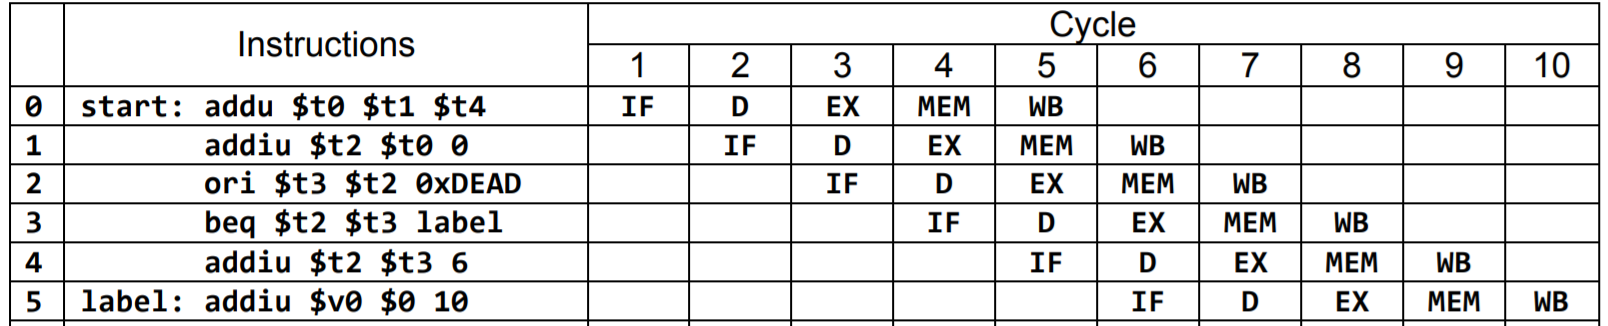
\includegraphics[width=\textwidth]{datapath/hazards}

\question Assume that this pipeline resolves control hazards by pipeline stalls. How many cycles is it stalled on a control hazard?

\begin{solution}[0.5in]
3 Cycles
\end{solution}

\question Should the pipeline stall for data hazards from load instructions? Give an example, fill in the corresponding pipeline stages, and explain your idea briefly in one or two sentences. 

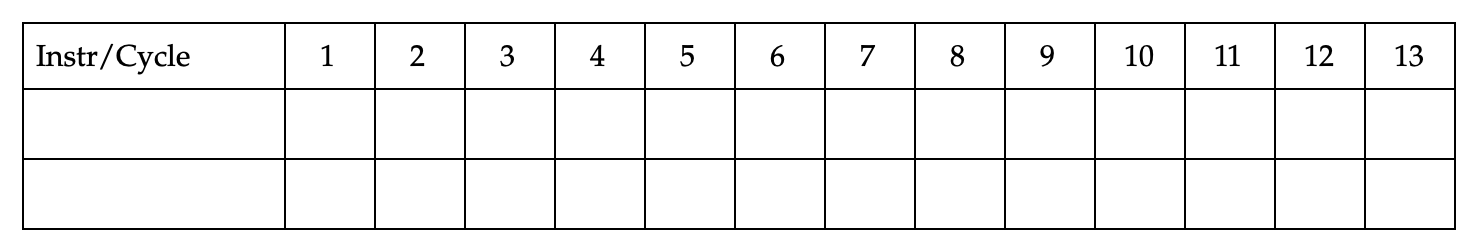
\includegraphics[width=\textwidth]{datapath/hazards_2}

\begin{solution}
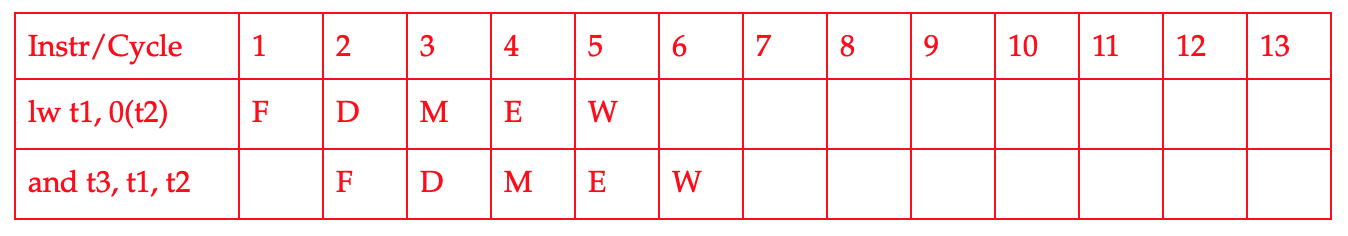
\includegraphics[width=\textwidth]{datapath/hazards_2_sol}
\end{solution}

\end{blocksection}